\section{Long-Context Speedrunning Track}
\label{sec:track2}

Speedrunning provides a natural optimization objective for long-horizon planning: a clear metric (completion time), decomposable milestones for fine-grained credit assignment, and a task that demands the full stack of AI capabilities---visual perception, long-horizon planning, persistent memory, spatial navigation, and strategic combat---simultaneously. We formalize RPG gameplay as an episodic MDP $\mathcal{M} = (\mathcal{S}, \mathcal{A}, T, R, \gamma)$ where actions are button inputs, transitions are largely deterministic for navigation but stochastic for battles, and reward is $+1$ per milestone with $\gamma = 1$.

\subsection{Speedrunning Environment Design}

The evaluation environment runs the game server at a fixed frame rate. Agents receive visual frames and limited state information---party composition (species, levels), status conditions, and HP values---but puzzle states, dynamic obstacles, items, and movesets are not exposed, so that perception remains challenging (see Figure~\ref{fig:track2_interface} in Appendix~\ref{sec:environment-details}).

\subsection{Speedrunning Evaluation Criteria}

Agents are evaluated on \textbf{completion percentage} (progress through standardized milestones, illustrated in Figure~\ref{fig:route}) and \textbf{completion time} for agents achieving 100\%, with ties broken by action count. An \textit{action} is each discrete instance where the agent outputs button presses to the emulator. We scoped the initial evaluation to defeating the first gym leader (Roxanne). Even this early segment requires thousands of agent steps and millions of reasoning tokens, with agents maintaining coherent plans across extended context windows that accumulate over hours of real-time play. The task demands the full stack of AI capabilities---perception, memory, planning, navigation, and battle strategy---and requires context compaction to manage the thousands of reasoning steps involved. We scope to the first gym to enable rapid iteration on approaches at reasonable cost; the milestone framework naturally extends to the full game as agent performance saturates.

\begin{figure}[t]
    \centering
    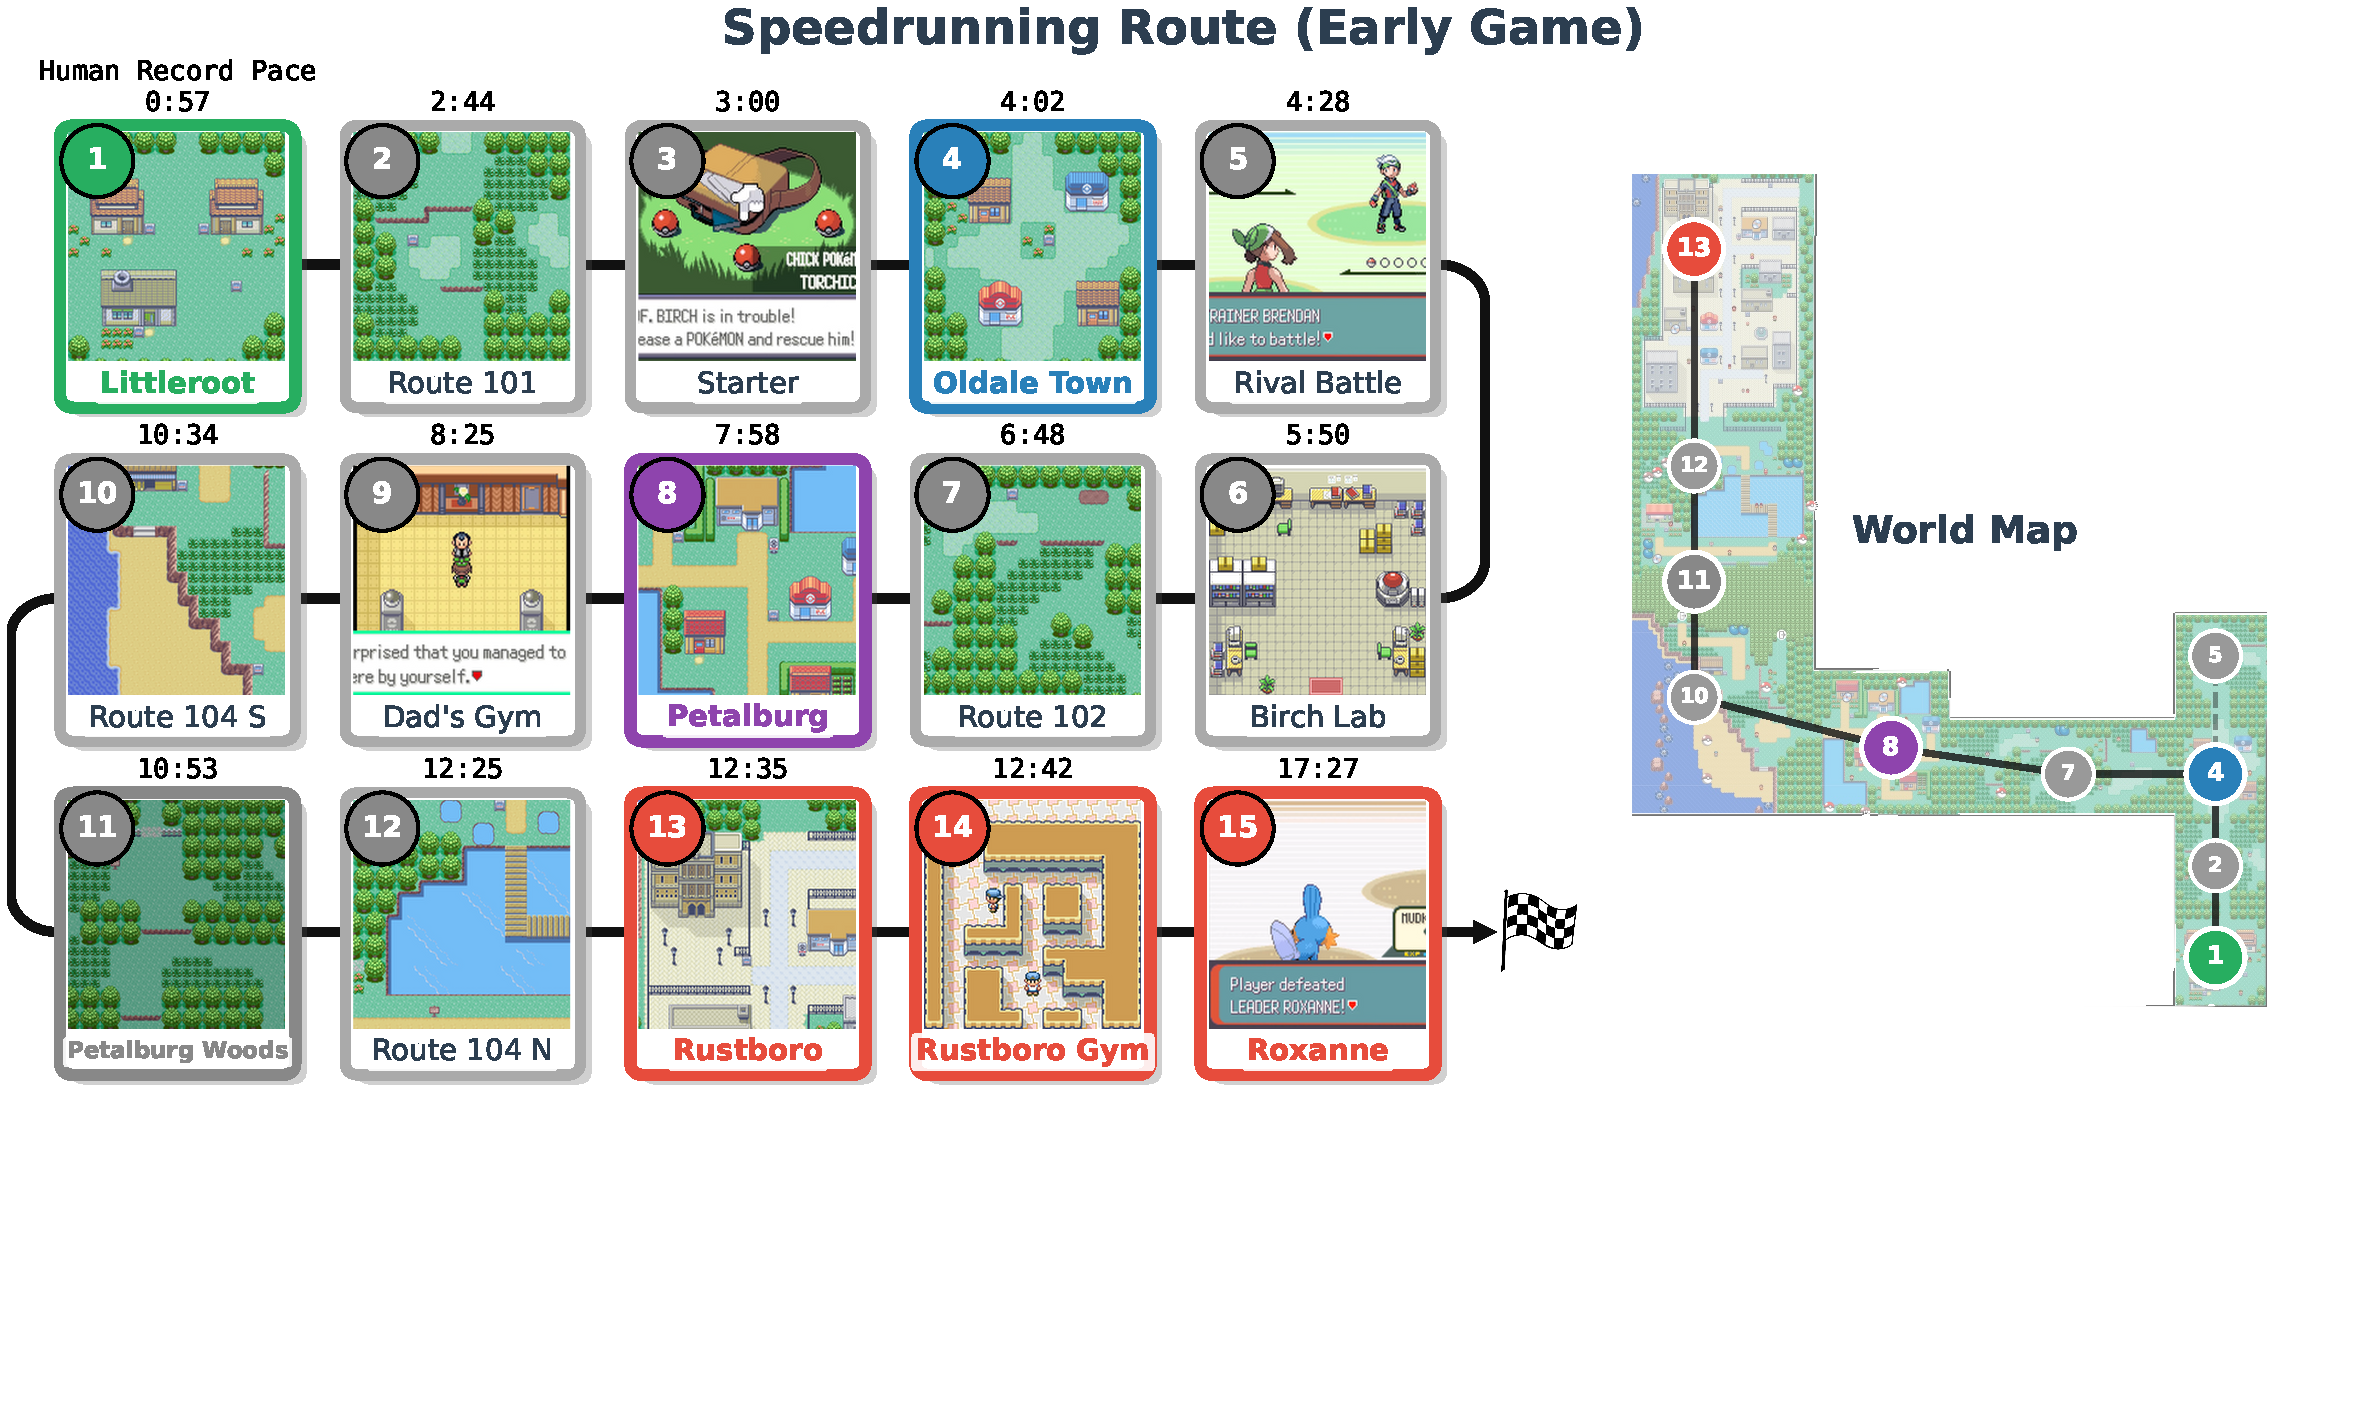
\includegraphics[width=.98\linewidth]{figures/speedrun_route.pdf}
    \vspace{-18mm}
    \caption{\textbf{Speedrunning Route (Early Game).} Milestones from \texttt{Littleroot Town} (1) to \texttt{Defeating Roxanne} (15), with game frames from each waypoint. The geographic overview (right) maps key locations. Although progression appears linear, the route requires substantial exploration and backtracking---agents must revisit earlier areas, navigate branching paths, and manage nonlinear dependencies between objectives. We provide splits from the human world record as an upper bound.}
    \vspace{-4mm}
    \label{fig:route}
\end{figure}

\vspace{-2mm}

\subsection{Speedrunning Baselines}

\paragraph{Human Baselines.} We scope evaluation to the first gym to enable participants to reasonably iterate on their approaches. Our top human speedrunner reached the first gym in 18 minutes, while average human players completed it in 1:22:05.

\vspace{-2mm}

\paragraph{Harness versus Model Capability.} A key challenge in evaluating LLM-based game agents is attribution: does performance stem from the underlying model or the surrounding harness (also called scaffold)? As discussed in Section~\ref{sec:intro}, prior efforts (Claude, Gemini, GPT playing Pokémon) conflated these factors. We disentangle them through a harness $\times$ model eval framework that analyzes systems along five dimensions---state representation ($S$), tools ($T$), memory ($M$), feedback ($F$), and fine-tuning ($\Phi$)---so that approaches can be compared on equal footing (Appendix \ref{sec:environment-details} Table~\ref{tab:system-comparison} and Figure~\ref{fig:track2_results}). Figure~\ref{fig:track2_results} compares our harness against common CLI-agent harnesses (Claude Code, Codex CLI, Gemini CLI) reveal that, while coding-agent architectures are  impressive out-of-the-box,  they nonetheless struggle to maintain coherence over the thousands of sequential decisions required for, and the non-linear exploration characteristic of RPG play.

\vspace{-2mm}

\paragraph{\pokeagent Baseline.} We release the first open-source multi-agent orchestration system for long-horizon RPG play. The system coordinates MCP tools (A* pathfinding, button inputs, knowledge retrieval) with specialized sub-agents for battle strategy, self-reflection, gym puzzles, and objective verification. A central orchestrator maintains a high-level route plan while dynamically dispatching sub-agents based on game context, with automatic context compaction to manage the thousands of reasoning steps required (see Appendix~\ref{sec:pokeagent-architecture} for architecture details). We evaluate five frontier models using the same harness (Figure~\ref{fig:track2_results}): Gemini 3 Flash achieves the fastest mean completion ($\sim$2:24), while Claude Sonnet 4.5 completes all milestones but with high variance (6:25--20:45 across runs). Even the best organizer baseline remains $\sim$1.8$\times$ slower than the average human (1:22:05).

\begin{figure}[t]
    \centering
    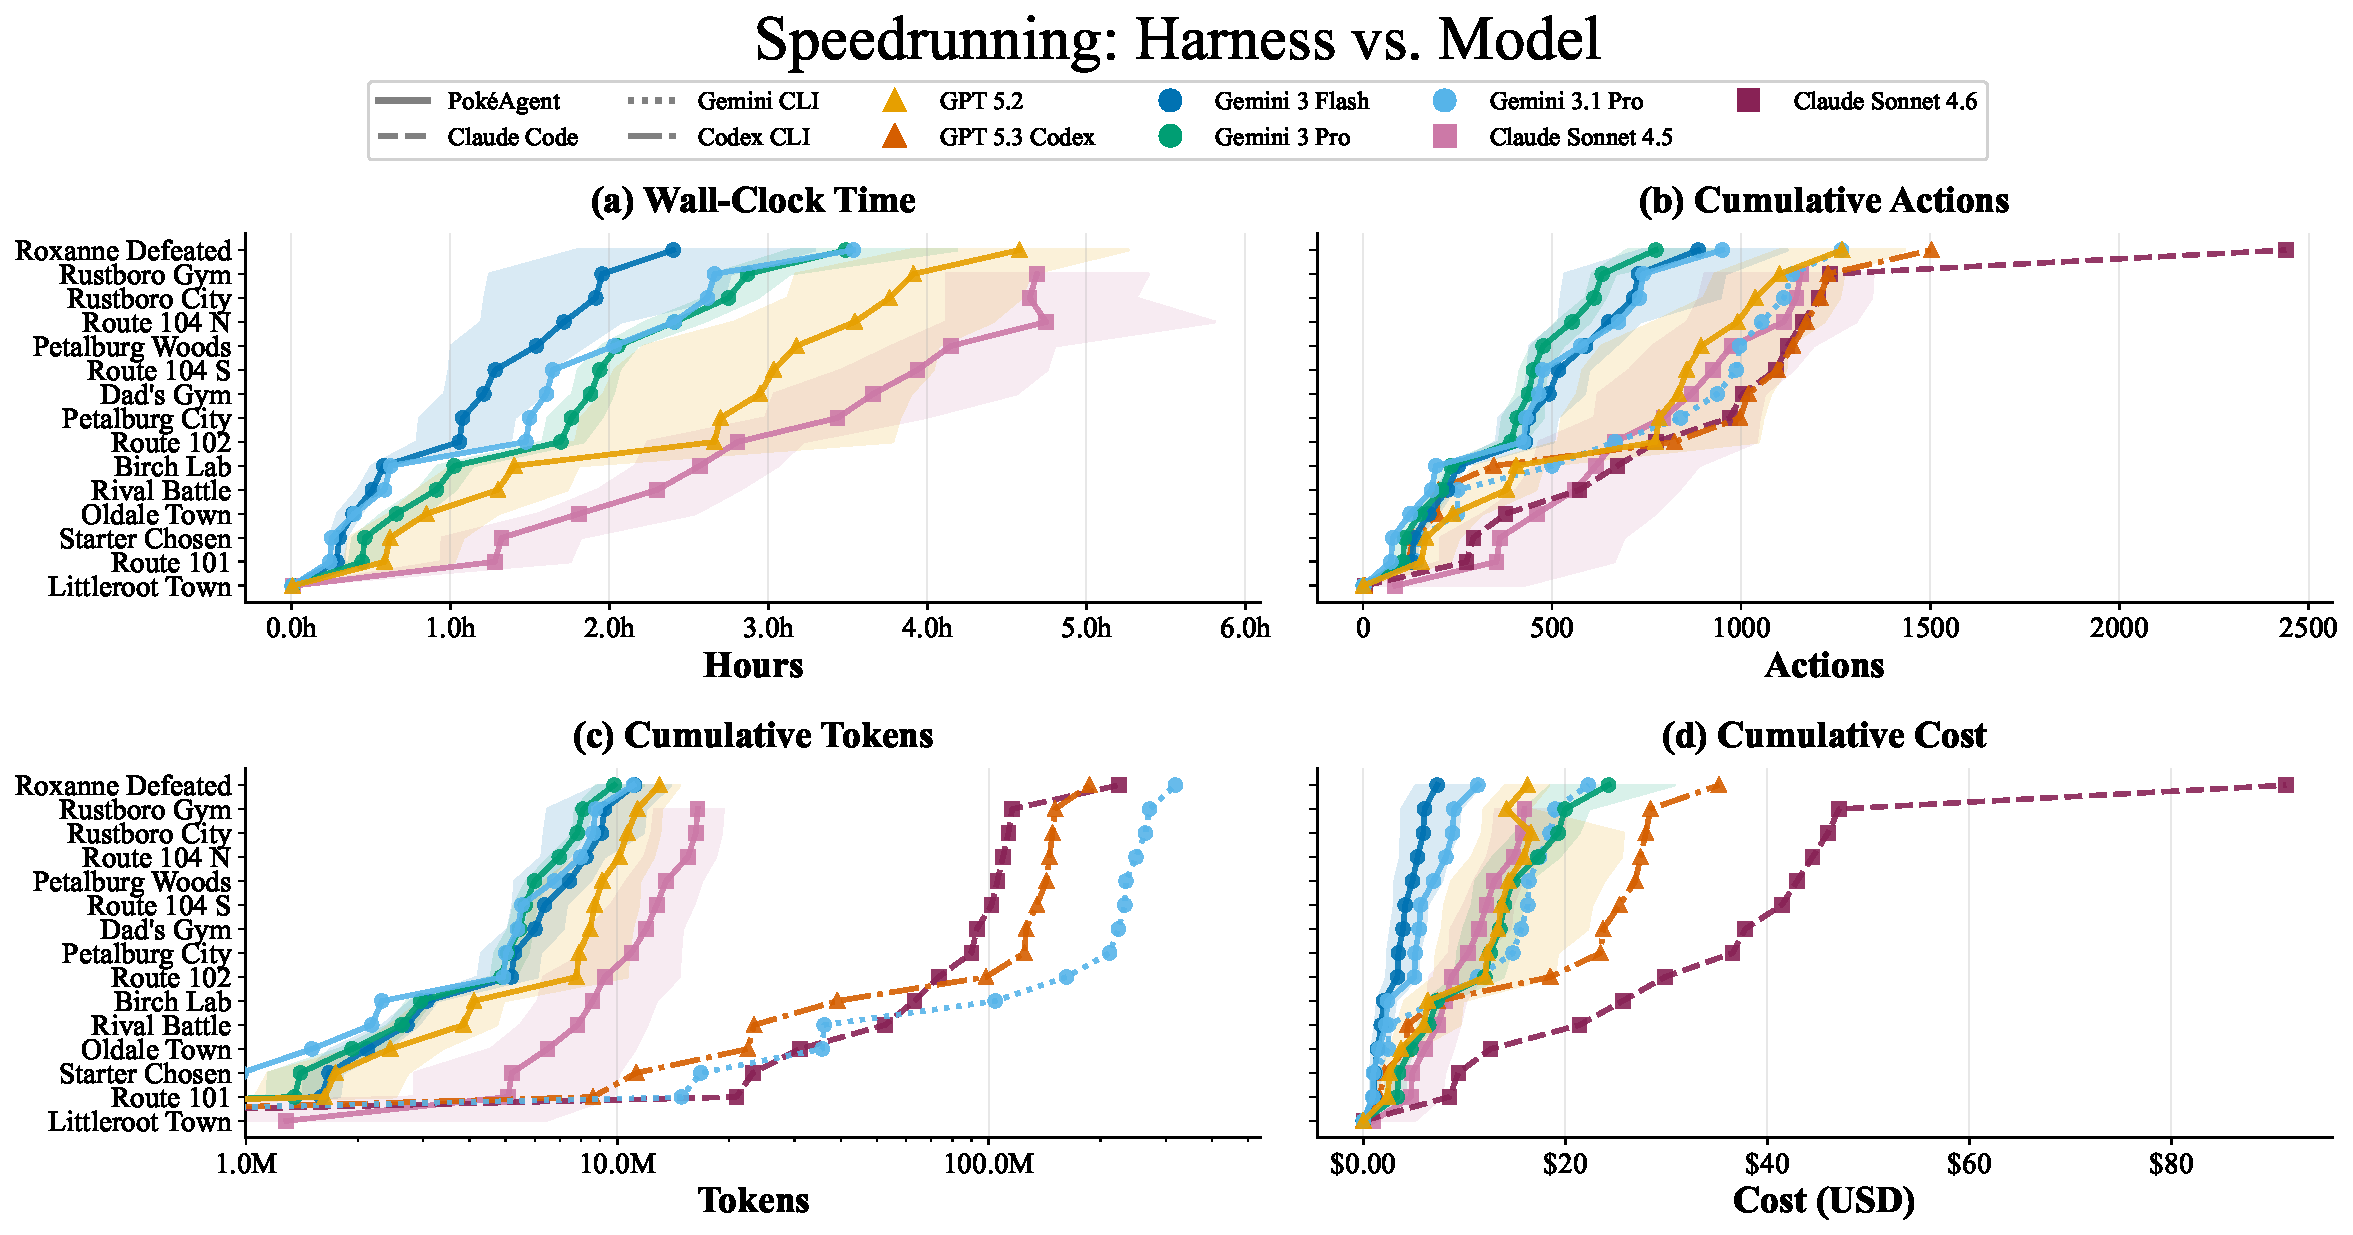
\includegraphics[width=.95\linewidth]{figures/milestone_confidence.pdf}
    \caption{\textbf{Speedrunning Track Baseline Results.} Cumulative wall-clock time, actions, tokens, and cost at each milestone for five frontier models (mean $\pm$ min/max range across runs). Gemini 3 Flash completes the route fastest ($\sim$2:24 mean) but requires more actions than Gemini 3 Pro. Claude Sonnet 4.5 completes all milestones but with the highest variance and 3--4$\times$ the cost of Gemini variants. GPT-5.2 falls between the two families in both time and cost.}
    \label{fig:track2_results}
\end{figure}
